\documentclass[aspectratio=169]{beamer}
\usepackage[utf8]{inputenc}
\usepackage{multicol}
\usepackage{tikz}

\title{Towards Pulverised Architectures for Collective Adaptive Systems through Multi-tier Programming}

\author[G.Aguzzi]{
  \textbf{Gianluca Aguzzi}\inst{1} \and
  Roberto Casadei\inst{1} \and
  Danilo Pianini\inst{1} \\
  Guido Salvaneschi\inst{2} \and
  Mirko Viroli\inst{1}
}
\institute{
  \inst{1}
  \texttt{Alma Mater Studiorum} -- Università di Bologna, Cesena, Italy \\
  \inst{2}
  University of St.Gallen: St.Gallen, Switzerland
}

\usetheme{material}
\useLightTheme
\usePrimaryTeal
\useAccentIndigo
%% TODO move out
\newcommand{\presentationGraphics}[3]{
  \begin{tikzpicture}
    \node[anchor=south west,inner sep=0] (B) at (4,0) {
      \cardImg{#1}{#3\textwidth}
       
    };
    \only<#2>{%
        \fill [draw=none, fill=white, fill opacity=0.7] (B.north west) -- (B.north east) -- (B.south east) -- (B.south west) -- (B.north west) -- cycle;
    }
  \end{tikzpicture}
}

\begin{document}

\begin{frameImg}{img/background.jpg}
\titlepage
\end{frameImg}

%\begin{frame}{Table of contents}
%\begin{card}
%\tableofcontents
%\end{card}
%\end{frame}

\section{Overview}
\begin{frameImg}{img/background.jpg}
\begin{card}[Collective Adaptive Systems]
\textit{a definition}
\end{card}
\end{frameImg}

\begin{frame}{Challenges}
%\only<1-4>{ \begin{backgroundblock} 
\includegraphics[width=\paperwidth]{img/network.jpg} \end{backgroundblock} }
%\only<5-6>{ \begin{backgroundblock} \includegraphics[width=\paperwidth]{example-image-a} \end{backgroundblock} }
\only<1-4>{ \begin{backgroundblock} 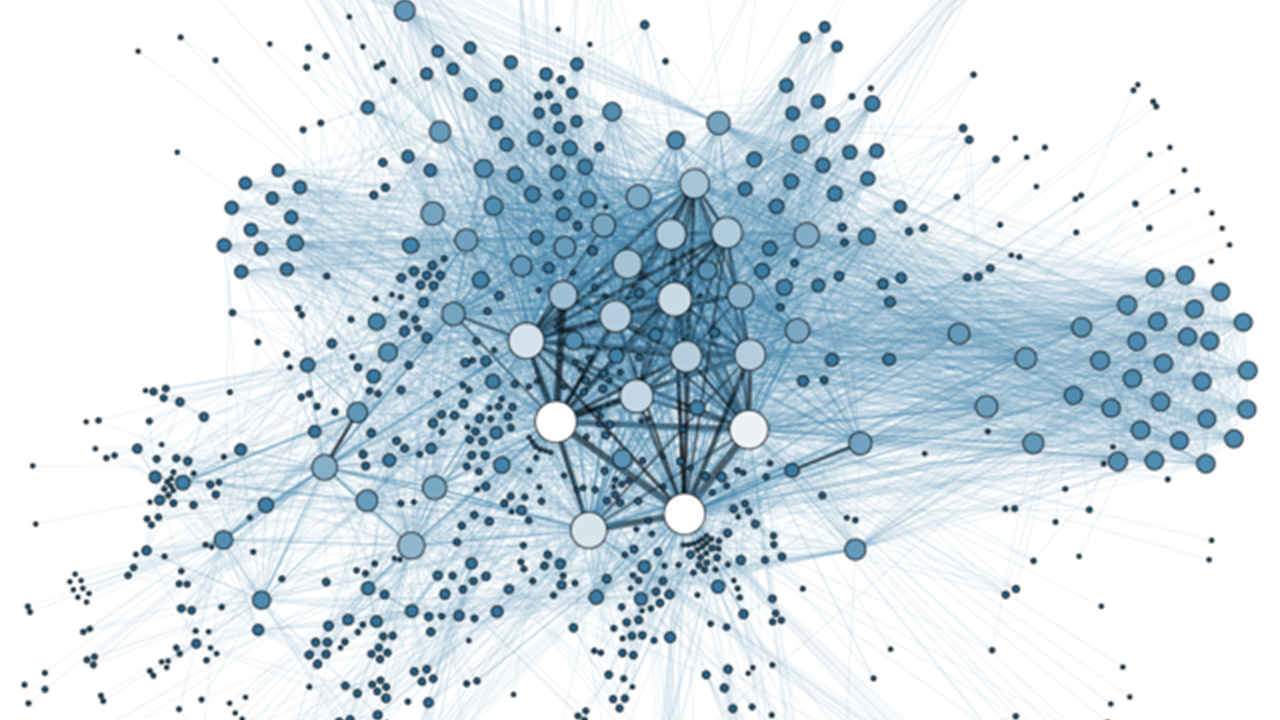
\includegraphics[width=\paperwidth]{img/complex-network.png} \end{backgroundblock} }
\only<5-6>{ \begin{backgroundblock} 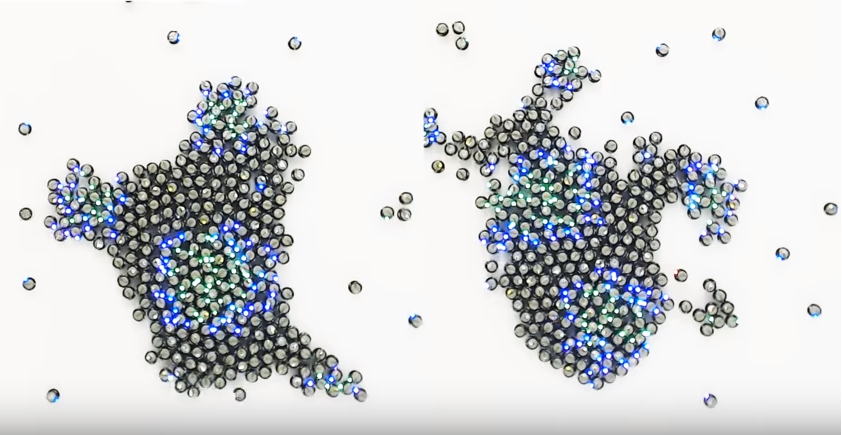
\includegraphics[height=\paperheight]{img/swarms.png} \end{backgroundblock} }

\begin{card}
{ 
  \setbeamercovered{transparent=10}
  \begin{itemize}
  \item<1-| alert@1> Complex and layered networks
  \begin{itemize}
    \item <2-| alert@2>Large scale
    \item <3-| alert@3>Heterogenous
    \item <4-| alert@4>Dynamic
  \end{itemize}
  \item<5-| alert@5> Distributed control
  \item<6-| alert@6> Environmental changes
  \end{itemize}
}

\end{card}
\end{frame}

\section{Proposed approach}
\begin{frame}{Proposed approach}

\begin{card}
{ 
  \setbeamercovered{transparent=10}
  \begin{itemize}
  \item<1-> Describe the collective behaviour via {\color{accent} \textit{Aggregate Computing}}
  \item<2-> Define you concrete deployment via {\color{accent} \textit{Multi-tier programming}}
  \item<3-> Inject the {\color{accent} \textit{same}} aggregate behaviour thanks to {\color{accent} \textit{Pulverisation}}
  \end{itemize}
}
\end{card}
\begin{multicols}{3}
\cardImg{example-image-a}{0.3\textwidth}
\presentationGraphics{example-image-b}{1}{0.3}
\presentationGraphics{example-image-c}{1-2}{0.3}
\end{multicols}
\end{frame}

\section{Aggregate Computing}
\begin{frame}{Aggregate Computing}
\begin{cardTiny}
{\color{accent} A top-down paradigm by wich programmers describe 
 a collective behaviour in a declarative and functional way,
 manipulating a distributed data structure called \textit{Computational field} }
\end{cardTiny}
\centering
\cardImg{example-image-b}{0.4\textwidth}
\end{frame}

\section{Pulverisation}
\begin{frame}{Pulverisation}

{
  \setbeamercovered{transparent=10}
  \begin{multicols}{2}
    [
      \begin{cardTiny}
      {\color{accent} An approach proposed for Aggregate Computing to neatly separate behavioural and deployment concerns. }
      \end{cardTiny}
    ]
    \centering
    \pause
    \presentationGraphics{img/logical-system.jpg}{1}{0.5}
    \pause
    \presentationGraphics{img/deployments}{1-2}{0.48}
    
    \end{multicols}
}

\end{frame}
\section{Multi-tier programming}

\begin{frame}{Multi-tier programming}
\begin{cardTiny}
{\color{accent} A programming apporach by with distributed architectures are defined in a single compilation unit with a single language. }
\end{cardTiny}
\centering
\cardImg{img/multitier}{0.4\textwidth}
\end{frame}

\section{Framework choosen}
\begin{frame}{Frameworks}%

{
  \setbeamercovered{transparent=10}
  \begin{card}[ScaFi (Scala Field)]
  A tool-chain composed by a Domain Specific Language that supports field-calculus.
  \end{card}
  \pause
  \begin{card}[ScalaLoci]
  A langauge extension to enable compile-time multi-tier programming.
  \end{card}
}
\end{frame}

\section{Puliverised architectures}
\begin{frame}{Puliverised architectures, logical system}

\end{frame}
\begin{frame}{Puliverised architectures, concrete examples}

\end{frame}
\section{Benefits}
\begin{frame}{Benefits}

\end{frame}

\end{document}
